\documentclass[UTF8, 10pt]{beamer}
 
% Chinese
\usepackage{CJKutf8}

% Font
\usepackage{bookman}
\usefonttheme{serif}
%\usepackage[T1]{fontenc}
%\usepackage{tgbonum}

% Other packages
\usepackage{appendixnumberbeamer}
\usepackage{latexsym, amsmath, xcolor, multicol, booktabs}
\usepackage{graphicx, listings, stackengine}
\usepackage{multirow}
\usepackage{hyperref}
\hypersetup{hidelinks,
	colorlinks=true,
	allcolors=black,
	pdfstartview=Fit,
	breaklinks=true}
% SUFE.sty
\usepackage{SUFE} 
% Bibtex
\usepackage[citestyle=authoryear-comp, 
			backend=bibtex, 
			bibstyle=numeric, 
%			sorting=ynt
			]{biblatex}
\setbeamertemplate{bibliography item}[text]
\addbibresource{ref.bib}

% Other setting


%%%%%%%%%%%%%%%%%%%%%%%%%%

% Title page
%% Author
\author[Haotian Deng] % The short name
{
Haotian Deng
\\
Jiangyuan Li
\\
Jinqiang Yang
%邓皓天
%\inst{1}
%\and
%Yuting Liu 
%\inst{2}
} 
%% Title & Subtitle
\title[High Frequency Evolution of Macro Expectation and Disagreement]{High Frequency Evolution of Macro Expectation and Disagreement}
\subtitle{}
%% Institution
\institute[SUFE]
{
%\inst{1}
Shanghai University of Finance and Economics
%上海财经大学金融学院
%\and
%\inst{2}
%Shanghai University of Finance and Economics
}
%% Date
\date[VLC 2021]
{\today}
%%Logo
%\logo{
\includegraphics[height=1cm]{sufe_logo}}

%%%%%%%%%%%%%%%%%%%%%%%%%%

% Document begins
\begin{document}
\begin{CJK*}{UTF8}{gbsn}

%Title page
\begin{frame}[noframenumbering]
%	\thispagestyle{empty}
	\titlepage
	% Logo
	\vspace{-0.5cm}
    \begin{figure}[htpb] 
        \begin{center}
            
\includegraphics[width=0.19 \linewidth]{sufe_logo.png}
        \end{center}  
    \end{figure}
\end{frame}

% Contents page
%\begin{frame}{Roadmap}
%	\tableofcontents[sectionstyle=show,
% 	subsectionstyle=show/shaded/hide,
% 	subsubsectionstyle=show/shaded/hide]
%\end{frame}

% Body

\section{Introduction}
\begin{frame}{Motivation}
	\begin{itemize}
		\item Traditional theories, such as \alert{FIRE}, suggest that there should be \alert{no disagreement} among agents (Muth, 1961; Lucas Jr, 1972).
		\item Empirical evidence shows \alert{persistent disagreement} among agents (Jonung, 1981).
		\item Models of \alert{information rigidity} offer compelling explanations for these observations.
		\item Central to these models is the important role of information—or ``\alert{news}''.
		\item The \alert{high-frequency} nature of this news and the \alert{low-frequency} survey data are \alert{misaligned}.
		\item Goal: develop a framework that can \alert{simultaneously integrate} high-frequency news with low-frequency survey data.
	\end{itemize}
\end{frame}
\begin{frame}{Literature: Evolution of Expectations and Disagreement}
	Evolution of Expectations
		\begin{itemize}
			\item Economic agents \alert{adjust their expectations} in response to \alert{newly acquired information}
				(Coibion and Gorodnichenko, 2015).
			\item This dynamic process of expectation adjustment occurs at a \alert{frequency} that \alert{significantly exceeds} that of conventional survey reports.
		\end{itemize}
	\\ \ \\
	Evolution of Disagreement
		\begin{itemize}
			\item Lahiri and Sheng (2008) estimate a Bayesian learning model to show three components of disagreement:
				\begin{enumerate}
					\item \alert{prior-mean} heterogeneity.
					\item the \alert{weights} attached to these priors.
					\item diverse \alert{interpretations} of new information.
				\end{enumerate}
			\item Several \alert{econometric issues} arise in the estimation of the evolution equation for disagreement (Hsiao and Pesaran, 2008; Lahiri and Sheng, 2008).
		\end{itemize}
\end{frame}
\begin{frame}{Literature: Mixed-Frequency Method}
	Previous methods (Ghysels and Wright, 2009; Andreou et al., 2013; Chaudhry and Oh, 2020):
		\begin{itemize}
			\item Mixed-Data Sampling Regression (\alert{MIDAS})
			\item Kalman Filter (\alert{KF})
			\item Reinforcement Learning (\alert{RL})
		\end{itemize}
	\\\ \\
	Shortcomings of previous methods:
		\begin{itemize}
			\item \alert{Estimation efficiency}: one may need to estimate many parameters, resulting in low estimation efficiency.
			\item \alert{Empirical performance}: due to model complexity and computational limitations, one may encounter a poor out-of-sample performance.
			\item \alert{Interpretability}: methods with good empirical performance are difficult to have a reasonable economic explanation.
		\end{itemize}
\end{frame}
\begin{frame}{This Paper}
	\begin{itemize}
		\item We develop a novel \alert{mixed-frequency} framework that enables the simultaneous analysis of \alert{high-frequency news} and \alert{low-frequency expectations}.
		\item By utilizing \alert{representative forecasters} as proxies for real-world agents, we demonstrate that the \alert{evolution of forecast disagreement} follows the equation:
			$$\mathrm{\sigma}\left(\mathbb{F}_{i, t+1}\left[x_{t+1}\right]\right)
					=  \mathrm{\sigma}\left(\mathbb{F}_{i, t}\left[x_{t+1}\right]\right)
					+ (\Delta\boldsymbol{\beta})^{\prime}\mathbf{r}_{t+1}
			$$
		\item We \alert{reconstruct the unobserved daily series of both expectations and disagreement} regarding macroeconomic growth that span the interval between two quarterly survey
releases.
	\end{itemize}
\end{frame}
\begin{frame}{Roadmap}
	Data and Variables
	\\ \ \\
	High-frequency Evolution of Expectations
	\\ \ \\
	High-frequency Evolution of Disagreement
	\\ \ \\
	Application: Construct Daily Measures of Both Aggregate Growth Expectations and Disagreement
\end{frame}

\section{Data}
\begin{frame}{Data}
	Growth Expectations: quarterly SPF surveys
	\begin{itemize}
		\item One-quarter ahead real GDP growth \alert{forecast}
			$$
			\mathbb{F}_{t}\left[x_{t+1}\right] = 100 \times
		    \left[
		    (\frac{\mathbb{F}_{t}\left[X_{t+1}\right]}{\mathbb{F}_{t}\left[X_{t}\right]})^4-1
		    \right]
			$$
		\item Real-time quarterly \alert{nowcast}
			$$
			\mathbb{F}_{t+1}\left[x_{t+1}\right] = 100 \times
		    \left[
		    (\frac{\mathbb{F}_{t+1}\left[X_{t+1}\right]}{X_{t}})^4-1
		    \right]
			$$
	\end{itemize}
	Asset Returns: proxies for new information
	\begin{itemize}
		\item We adopt a \alert{broad interpretation} to asset prices, encompassing rate changes, spreads,
returns, and other value-related metrics of financial assets.
	\end{itemize}
\end{frame}

\section{High-Frequency Expectations}
\begin{frame}{Relation between News and Growth Expectations}
	\begin{itemize}
		\item The \alert{DGP} is defined by $x_{t}=\rho x_{t-1}+u_{t}$, where $u_{t} \sim \mathcal{N}\left(0, \sigma_{u}^{2}\right)$ is i.i.d. over time and $\rho>0$.
		\item Agent $i$ observes the \alert{noise signal} $s_{t}^{i}=x_{t}+\epsilon_{t}^{i}$, where $\epsilon_{t}^{i} \sim \mathcal{N}\left(0, \sigma_{\epsilon}^{2}\right)$ represents forecaster-specific i.i.d. noise.
		\item According to the \alert{Kalman filter}, beliefs should be updated as follows
			$$
			\underbrace{\mathbb{F}_{i, t+1}\left[x_{t+1}\right]}
			    _{\text{nowcast}}
			    =\underbrace{\mathbb{F}_{i, t}\left[x_{t+1}\right]}
			    _{\text{forecast}}
			    +\frac{\Sigma}{\Sigma+\sigma_{\epsilon}^{2}}\underbrace{
			\left(s_{t}^{i}-\mathbb{F}_{i, t}\left[x_{t+1}\right]\right)
			}_{\text{new information}}
			$$
			where $\Sigma$ is the steady state variance of the prior $f(x_{t+1}\mid s_t^i, s_{t-1}^i,\cdots)$.
		\item To help with interpretation of this equation, we transform it into a simpler form:
			$$
			\mathbb{F}_{i, t+1}\left[x_{t+1}\right]
    		= \mathbb{F}_{i, t}\left[x_{t+1}\right]
    		+ \textit{News}_{t+1}
			$$
			we interpret it as an \alert{efficient Bayesian forecaster}.
	\end{itemize}
\end{frame}
\begin{frame}{Relation between News and Growth Expectations}
	\begin{itemize}
		\item We need a model that allows for \alert{heterogeneity} without making any specific assumptions:
			$$
			\begin{aligned}
			\mathbb{F}_{i, t+1}\left[x_{t+1}\right]
		    &= \alpha_i \mathbb{F}_{i, t}\left[x_{t+1}\right]
		    + \boldsymbol{\beta}_i^{\prime}\mathbf{r}_{t+1}
		    \\
		    FR_{i, t+1} \equiv
		    \mathbb{F}_{i, t+1}\left[x_{t+1}\right] - \mathbb{F}_{i, t}\left[x_{t+1}\right]
		    &= (\alpha_i-1) \mathbb{F}_{i, t}\left[x_{t+1}\right]
		    + \boldsymbol{\beta}_i^{\prime}\mathbf{r}_{t+1}
		    \end{aligned}
			$$
		\item Motivated by this expression, we employ the following approximating moment:
			$$
			\mathbb{F}_{t+1}\left[x_{t+1}\right]
		    = \alpha \mathbb{F}_{t}\left[x_{t+1}\right] 
		    + \boldsymbol{\beta}^{\prime}\mathbf{r}_{t+1}
			$$
			where $\mathbf{r}_{t+1}$ represents a vector of \alert{asset returns},
			since they contain informative content for forecast revisions.
		\item We conduct several time series regressions to reinforce our use of \alert{asset returns as proxies for news}, since we observe that certain pairs of assets yield sizable $R^2$.
	\end{itemize}
\end{frame}
\begin{frame}{Mixed-Frequency Estimation Method}
	\begin{itemize}
		\item We encounter the \alert{issue with mixed frequencies}: forecasts are made quarterly, while the asset returns that represent news are recorded daily.
		\item A \alert{recursive form} of the evolution equation:
			$$
			\begin{aligned}
		       \mathbb{F}_{1}\left[x\right]
		        & = \alpha \mathbb{F}_{0}\left[x\right] 
		        + \boldsymbol{\beta}^{\prime}\mathbf{r}_{1} 
		        \\
		        \mathbb{F}_{2}\left[x\right]
		        & = \alpha \mathbb{F}_{1}\left[x\right] 
		        + \boldsymbol{\beta}^{\prime}\mathbf{r}_{2} 
		        \\
		        &\cdots
		        \\
		        \mathbb{F}_{T}\left[x\right]
		        & = \alpha \mathbb{F}_{T-1}\left[x\right] 
		        + \boldsymbol{\beta}^{\prime}\mathbf{r}_{T}
		    \end{aligned}
			$$
		\item This recursive approach allows us to clearly establish the relationship between $\mathbb{F}_{0}\left[x\right]$ and $\mathbb{F}_{T}\left[x\right]$ for two consecutive release dates:
			$$
			\mathbb{F}_{T}\left[x^p\right]
		    = \alpha^T \mathbb{F}_{0}\left[x^p\right]
		    + \sum_{k=0}^{T-1} \alpha^k \boldsymbol{\beta}^{\prime}\mathbf{r}_{T-k}^p
			$$
	\end{itemize}
\end{frame}
\begin{frame}{Mixed-Frequency Estimation Method}
	\begin{itemize}
		\item By setting $\alpha$ to \alert{a fixed value $\alpha_0$}, we simplify the equation and therefore allow it to estimate using OLS:
			$$
			\mathbb{F}_{T}\left[x^p\right]
		    - \alpha_0^T \mathbb{F}_{0}\left[x^p\right]
		    = \boldsymbol{\beta}^{\prime} (\sum_{k=0}^{T-1} \alpha_0^k \mathbf{r}_{T-k}^p)
			$$
			Let $y=\mathbb{F}_{T}\left[x^p\right] - \alpha_0^T \mathbb{F}_{0}\left[x^p\right]$ and $\mathbf{X}=\sum_{k=0}^{T-1} \alpha_0^k \mathbf{r}_{T-k}^p$.
			\\
			Then, the estimator $\hat{\boldsymbol{\beta}}$ is given by $\hat{\boldsymbol{\beta}}=(\mathbf{X}^\prime \mathbf{X})^{-1}\mathbf{X}^\prime y$.
		\item Our current task is to identify the value of $\alpha_0$ that \alert{minimizes the $\mathrm{SSR}$}:
			$$
			\begin{aligned}
		        \frac{\partial \mathrm{SSR}}{\partial \alpha_{0}}
		        &= 2 T \alpha_{0}^{T-1} \mathbb{F}_{0}\left[x^{p}\right] \mathbf{X} \hat{\boldsymbol{\beta}}
		        - 2 y^{\prime}\left(\sum_{k=0}^{T-1} k \alpha_{0}^{k-1} \mathbf{r}_{T-k}^{p}\right) \hat{\boldsymbol{\beta}}
		        \\
		        & \quad + \hat{\boldsymbol{\beta}}^{\prime}\left[\left(\sum_{k=0}^{T-1} k \alpha_{0}^{k-1} \mathbf{r}_{T-k}^{p}\right)^{\prime} \mathbf{X}
		        +\mathbf{X}^{\prime}\left(\sum_{k=0}^{T-1} k \alpha_{0}^{k-1} \mathbf{r}_{T-k}^{p}\right)\right] \hat{\boldsymbol{\beta}}
		    \end{aligned}
			$$
	\end{itemize}
\end{frame}
\begin{frame}{Mixed-Frequency Estimation Method}
	We develop a \alert{grid search method} to identify the optimal $\alpha$:
	\begin{enumerate}
		\item We construct a grid over the \alert{feasible domain} of $\alpha$ and divide it into discrete intervals.
			\begin{itemize}
				\item Each grid point corresponds to a potential value of $\alpha$.
				\item The domain for $\alpha$ is based on theoretical considerations.
				\item We begin by setting a broad sampling range for $\alpha$ and gradually narrowing the interval to enhance accuracy.
			\end{itemize}
		\item We employ a \alert{rolling window} of 40 quarters.
			\begin{itemize}
				\item The parameters cannot remain constant.
				\item The window size should be carefully chosen to balance statistical power and parameter stability.
			\end{itemize}
		\item We restrict our analysis to \alert{bivariate pairs of assets}.
			\begin{itemize}
				\item A linear combination of two assets may approximate others.
				\item We specifically choose those that yield the highest $R^2$.
			\end{itemize}
	\end{enumerate}
\end{frame}
\begin{frame}{Estimation Results}
	\center The optimal coefficient $\alpha$ that minimize $\mathrm{SSR}$ is $1$.
	\begin{figure}[htpb]
	  \begin{center}
	    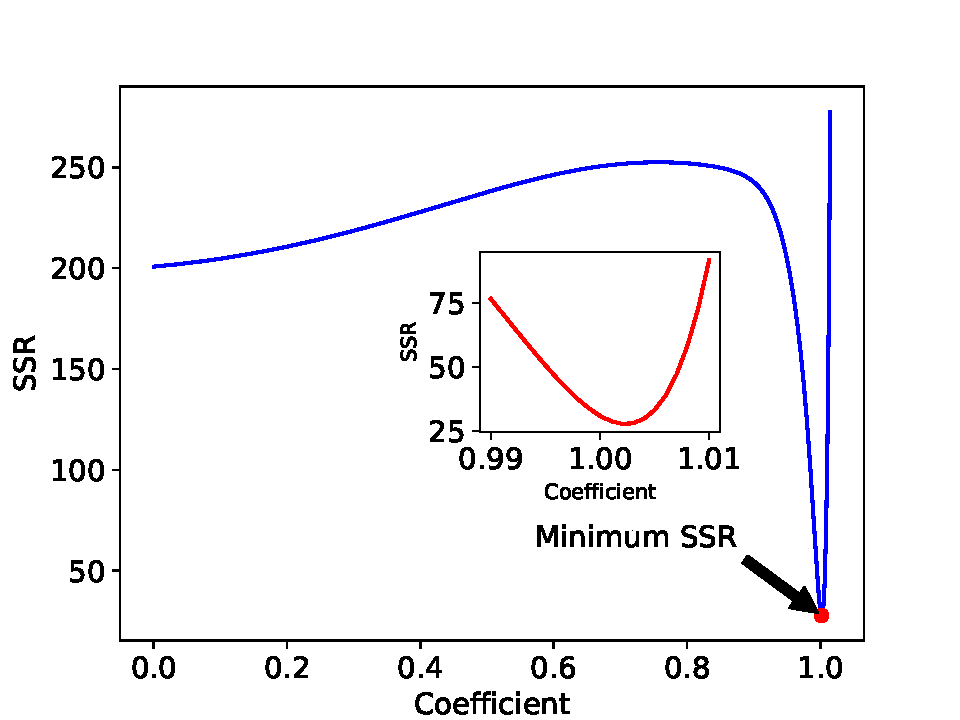
\includegraphics[width=0.7 \linewidth]
	    {pic/Figure_1.pdf}
	    \caption{Relationship between $\mathrm{SSR}$ and $\alpha$.}
	  \end{center}
	\end{figure}
\end{frame}
\begin{frame}{Estimation Results}
	$$
	FR^p \equiv
    \mathbb{F}_{T}\left[x^p\right] - \mathbb{F}_{0}\left[x^p\right]
    = \boldsymbol{\beta}^{\prime} (\sum_{k=0}^{T-1} \mathbf{r}_{T-k}^p)
    + (k \mathbb{F}_{0}\left[x^p\right] + b)
	$$
	\begin{table}[H]
    \centering
%    \caption{Regressions of equation}
    \label{Table4}
%    \begin{threeparttable}
        \begin{tabular}{l c c}
            \toprule
             & (1)& (2)\\
            \midrule
            \multirow{2}{*}{$\beta_1$ (5YR Fixed-term Index)}
            & -0.235*** & -0.362*** \\
            & (0.074) & (0.128) \\
            \multirow{2}{*}{$\beta_2$ (Change in AAA-10Y Spread)}
            & 0.024* & 0.035* \\
            & (0.013) & (0.019) \\
            \multirow{2}{*}{$b$ (constant)}
            &  & 0.609   \\
            &  & (0.636)   \\
            \multirow{2}{*}{$k$ (past forecast $\mathbb{F}_{0}\left[x^p\right]$)}
            &  & -0.086 \\
            &  & (0.253) \\
            $R^2$ & 0.224 & 0.280  \\
        \bottomrule
        \end{tabular}
%    \end{threeparttable}
	\end{table}
\end{frame}

\section{High-Frequency Disagreement}
\begin{frame}{Intuition}
	\begin{itemize}
		\item The \alert{cross-sectional variance} is defined as 
			$$
			\mathrm{Var}(\mathbb{F}_{i, t}\left[x_{t+1}\right]) = \frac{1}{N}\sum_{i=1}^N (\mathbb{F}_{i, t}\left[x_{t+1}\right]-\mathbb{F}_{t}\left[x_{t+1}\right])^2
			$$
		\item By incorporating the \alert{evolution equations} for both individual and consensus forecasts:
			$$
			\mathrm{Var}(\mathbb{F}_{i, t+1}\left[x_{t+1}\right])
		    =
		    \gamma \mathrm{Var}(\mathbb{F}_{i, t}\left[x_{t+1}\right])
		    + \boldsymbol{\zeta}^{\prime} \mathbf{r}_{t+1} \mathbf{r}_{t+1}^\prime \boldsymbol{\zeta}
		    +
		    \boldsymbol{\delta}^\prime \mathbf{r}_{t+1} \mathbb{F}_{t}\left[x_{t+1}\right]
			$$
			where $\gamma$ is a scalar related to $\alpha$ and $\alpha_i$, $\boldsymbol{\zeta}$ is a vector of scalars related to $\boldsymbol{\beta}$ and $\boldsymbol{\beta}_i$, and $\boldsymbol{\delta}$ is a vector of scalars related to $\alpha$, $\alpha_i$, $\boldsymbol{\beta}$, and $\boldsymbol{\beta}_i$.
		\item If we \alert{relax these constraints} and apply the previous method, the results, although computable, do not reflect the \alert{true ``variance'' parameters} as needed.
	\end{itemize}
\end{frame}
\begin{frame}{Representative Forecasters}
	\begin{itemize}
		\item We posit the existence of two such forecasters:
			$$
			\begin{aligned}
		        \mathbb{F}_{t}^{H}\left[x_{t+1}\right]
		        & = \mathbb{F}_{t}\left[x_{t+1}\right] + \mathrm{\sigma}\left(\mathbb{F}_{i, t}\left[x_{t+1}\right]\right)
		        \\
		        \mathbb{F}_{t}^{L}\left[x_{t+1}\right]
		        & = \mathbb{F}_{t}\left[x_{t+1}\right] - \mathrm{\sigma}\left(\mathbb{F}_{i, t}\left[x_{t+1}\right]\right)
		    \end{aligned}
			$$
			we assume that the \alert{position} of representative forecasts in relation to consensus forecast \alert{remains constant} over time.
		\item Since we have
			$$
			\begin{aligned}
%				\mathbb{F}_{t+1}\left[x_{t+1}\right]
%				    & = \alpha \mathbb{F}_{t}\left[x_{t+1}\right] + \boldsymbol{\beta}^{\prime}\mathbf{r}_{t+1}
%			    \\
			    \mathbb{F}^H_{t+1}\left[x_{t+1}\right]
			    & = \alpha^H \mathbb{F}_{t}^H\left[x_{t+1}\right] + (\boldsymbol{\beta}^H)^{\prime}\mathbf{r}_{t+1}
			    \\
			    \mathbb{F}^L_{t+1}\left[x_{t+1}\right]
			    & = \alpha^L \mathbb{F}_{t}^L\left[x_{t+1}\right] + (\boldsymbol{\beta}^L)^{\prime}\mathbf{r}_{t+1}
			\end{aligned}
			$$
		\item The \alert{relationship} between representative forecasters and consensus is
			$$
			\begin{aligned}
		        2 \mathbb{F}_{t+1}\left[x_{t+1}\right]
		        & =
		        \mathbb{F}_{t+1}^{H}\left[x_{t+1}\right] + \mathbb{F}_{t+1}^{L}\left[x_{t+1}\right]
		        \\
		        2 \alpha \mathbb{F}_{t}\left[x_{t+1}\right] 
		        + 2 \boldsymbol{\beta}^{\prime}\mathbf{r}_{t+1}
		        & = 
		        (\alpha^H+\alpha^L) \mathbb{F}_{t}\left[x_{t+1}\right]
		        +
		        \left[(\boldsymbol{\beta}^H)^{\prime}+(\boldsymbol{\beta}^L)^{\prime}\right]\mathbf{r}_{t+1}
		        \\
		        &\quad +
		        (\alpha^H-\alpha^L) \mathrm{\sigma}\left(\mathbb{F}_{i, t}\left[x_{t+1}\right]\right)
		    \end{aligned}
			$$
	\end{itemize}
\end{frame}
\begin{frame}{Learning the Cross-sectional Variance}
	\begin{itemize}
		\item Drawing from the conclusion that $\alpha^H=\alpha^L=\alpha=1$:
			$$
			\begin{aligned}
		        \left[
		        \mathbb{F}_{t+1}\left[x_{t+1}\right] + \mathrm{\sigma}\left(\mathbb{F}_{i, t+1}\left[x_{t+1}\right]\right)
		        \right]
		        & = 
		        \left[
		        \mathbb{F}_{t}\left[x_{t+1}\right] + \mathrm{\sigma}\left(\mathbb{F}_{i, t}\left[x_{t+1}\right]\right)
		        \right]
		        + (\boldsymbol{\beta}^H)^{\prime}\mathbf{r}_{t+1}
		        \\
		        \mathbb{F}_{t+1}\left[x_{t+1}\right]
		        & = 
		        \mathbb{F}_{t}\left[x_{t+1}\right]
		        + \boldsymbol{\beta}^{\prime}\mathbf{r}_{t+1}
		        \\
		        \left[
		        \mathbb{F}_{t+1}\left[x_{t+1}\right] - \mathrm{\sigma}\left(\mathbb{F}_{i, t+1}\left[x_{t+1}\right]\right)
		        \right]
		        & = 
		        \left[
		        \mathbb{F}_{t}\left[x_{t+1}\right] - \mathrm{\sigma}\left(\mathbb{F}_{i, t}\left[x_{t+1}\right]\right)
		        \right]
		        + (\boldsymbol{\beta}^L)^{\prime}\mathbf{r}_{t+1}
		    \end{aligned}
			$$
		\item It becomes apparent that the cross-sectional standard deviation follows a straightforward evolution equation
			$$
			\mathrm{\sigma}\left(\mathbb{F}_{i, t+1}\left[x_{t+1}\right]\right)
    		= 
		    \alpha \mathrm{\sigma}\left(\mathbb{F}_{i, t}\left[x_{t+1}\right]\right)
		    + (\Delta\boldsymbol{\beta})^{\prime}\mathbf{r}_{t+1}
			$$
			where $\Delta \boldsymbol{\beta} = \boldsymbol{\beta}^H - \boldsymbol{\beta} = \boldsymbol{\beta} - \boldsymbol{\beta}^L$ represent the \alert{differential interpretation of news} between two representative forecasts and the consensus forecast.
	\end{itemize}
\end{frame}
\begin{frame}{Discussion}
	\begin{itemize}
		\item We now turn to a more general case:
			$$
		        \mathbb{F}_{i, t}\left[x_{t+1}\right]
		        = \mathbb{F}_{t}\left[x_{t+1}\right] + k_i\cdot \mathrm{\sigma}\left(\mathbb{F}_{i, t}\left[x_{t+1}\right]\right)
			$$
			where $k_i\neq 0$ \alert{remains constant over time}.
		\item By substituting it into the evolution equation for individuals and consensus:
			$$
			\mathrm{\sigma}\left(\mathbb{F}_{i, t+1}\left[x_{t+1}\right]\right)
	        =\alpha_i \mathrm{\sigma}\left(\mathbb{F}_{i, t}\left[x_{t+1}\right]\right)
	        +\frac{\alpha_i-\alpha}{k_i}\mathbb{F}_{t}\left[x_{t+1}\right]
	        +(\frac{\boldsymbol{\beta}_i-\boldsymbol{\beta}}{k_i})^\prime \mathbf{r}_{t+1}
			$$
		\item Notice that this equation holds for any representative forecaster $i$, substitute $\alpha_i=\alpha$:
			$$
			\mathrm{\sigma}\left(\mathbb{F}_{i, t+1}\left[x_{t+1}\right]\right)
	        =\alpha \mathrm{\sigma}\left(\mathbb{F}_{i, t}\left[x_{t+1}\right]\right)
	        +(\frac{\boldsymbol{\beta}_i-\boldsymbol{\beta}}{k_i})^\prime \mathbf{r}_{t+1}
			$$
			This is equivalent to the evolution equation we derive previously, where $\Delta\boldsymbol{\beta}=(\boldsymbol{\beta}_i-\boldsymbol{\beta})/k_i$.
	\end{itemize}
\end{frame}
\begin{frame}{Estimation Results}
	\center The optimal $\alpha$ that minimize $\mathrm{SSR}$ for disagreement is also $1$.
	\begin{figure}[htpb]
	  \begin{center}
	    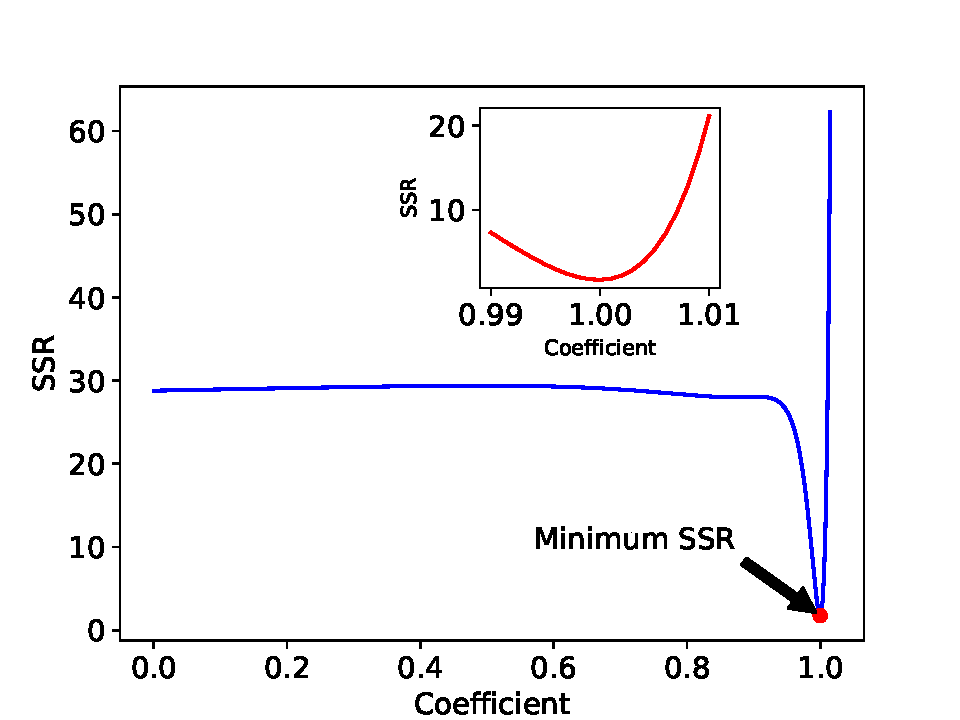
\includegraphics[width=0.7 \linewidth]
	    {pic/Figure_5.pdf}
	    \caption{Relationship between $\mathrm{SSR}$ and $\alpha$ for disagreement.}
	  \end{center}
	\end{figure}
\end{frame}

\section{Application}
\begin{frame}{Extract Daily Time Series of Mean and Variance}
	Applying the previous mixed-frequency method, we derive the estimated daily-frequency time series:
			$$
			\left[\begin{array}{c}\mathbb{F}_{1}\left[x^{p}\right] \\ \mathbb{F}_{2}\left[x^{p}\right] \\ \vdots \\ \mathbb{F}_{T}\left[x^{p}\right]\end{array}\right]=\mathbf{D}\left[\begin{array}{c}\mathbb{F}_{0}\left[x^{p}\right] \\ \mathbb{F}_{0}\left[x^{p}\right] \\ \vdots \\ \mathbb{F}_{0}\left[x^{p}\right]\end{array}\right]+\mathbf{T}\left[\begin{array}{c}\mathbf{r}_{1}^{p} \\ \mathbf{r}_{2}^{p} \\ \vdots \\ \mathbf{r}_{T}^{p}\end{array}\right]
			$$
	where $\mathbf{D}=\operatorname{diag}\left(\hat{\alpha}^{1}, \hat{\alpha}^{2}, \cdots, \hat{\alpha}^{T}\right)$ is a scaling matrix that represents the contribution of the initial state $\mathbb{F}_{0}\left[x^{p}\right]$.
	$\mathbf{T}$ is a Toeplitz matrix that expresses the impact of asset returns:
	$$
	\mathbf{T}=\left[\begin{array}{c c c c}\hat{\boldsymbol{\beta}}^{\prime} & 0 & \cdots & 0 \\ \hat{\alpha} \hat{\boldsymbol{\beta}}^{\prime} & \hat{\boldsymbol{\beta}}^{\prime} & \cdots & 0 \\ \vdots & \vdots & \ddots & \vdots \\ \hat{\alpha}^{T-1} \hat{\boldsymbol{\beta}}^{\prime} & \hat{\alpha}^{T-2} \hat{\boldsymbol{\beta}}^{\prime} & \cdots & \hat{\boldsymbol{\beta}}^{\prime}\end{array}\right]
	$$
\end{frame}
\begin{frame}{Results}
	Recursive estimation:
	\begin{itemize}
		\item We fit model on previous $T-1$ quarters and apply to one quarter out-of-sample.
	\end{itemize}
	Evaluation:
	\begin{itemize}
		\item We construct the daily series for both cross-sectional mean and variance and achieve impressive $R^2$ of 93.3\% and 84.5\% against the actual data from surveys.
	\end{itemize}
	\begin{columns}
		\column{0.5\textwidth}
		\begin{figure}[htpb]
		  \begin{center}
		    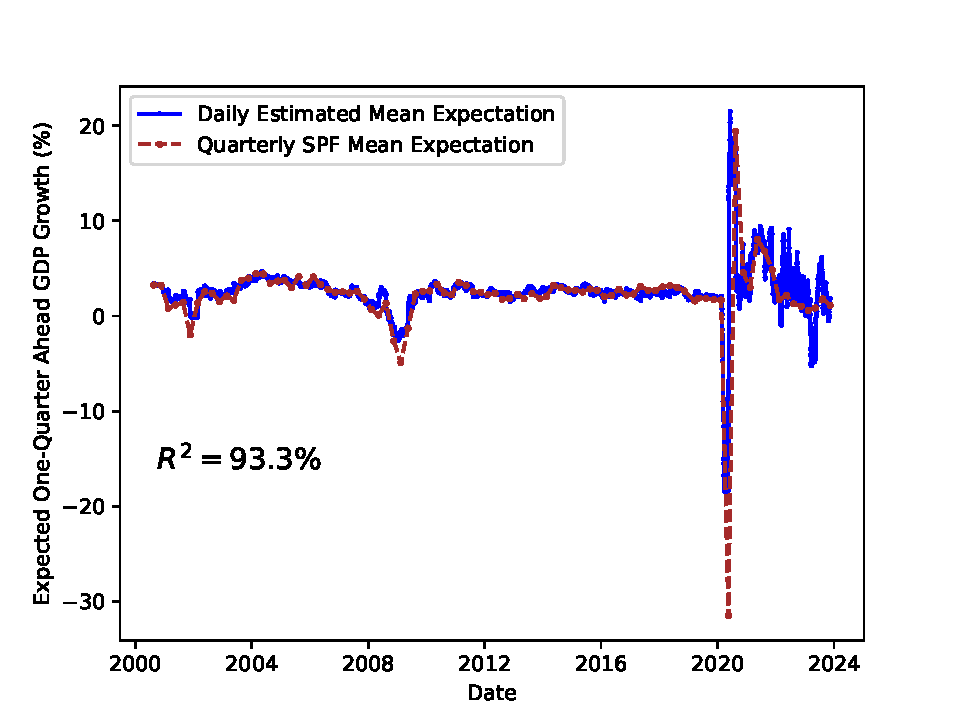
\includegraphics[width=0.8 \linewidth]
		    {pic/Figure_6.pdf}
		    \caption{Expectations}
		  \end{center}
		\end{figure}
		\column{0.5\textwidth}
		\begin{figure}[htpb]
		  \begin{center}
		    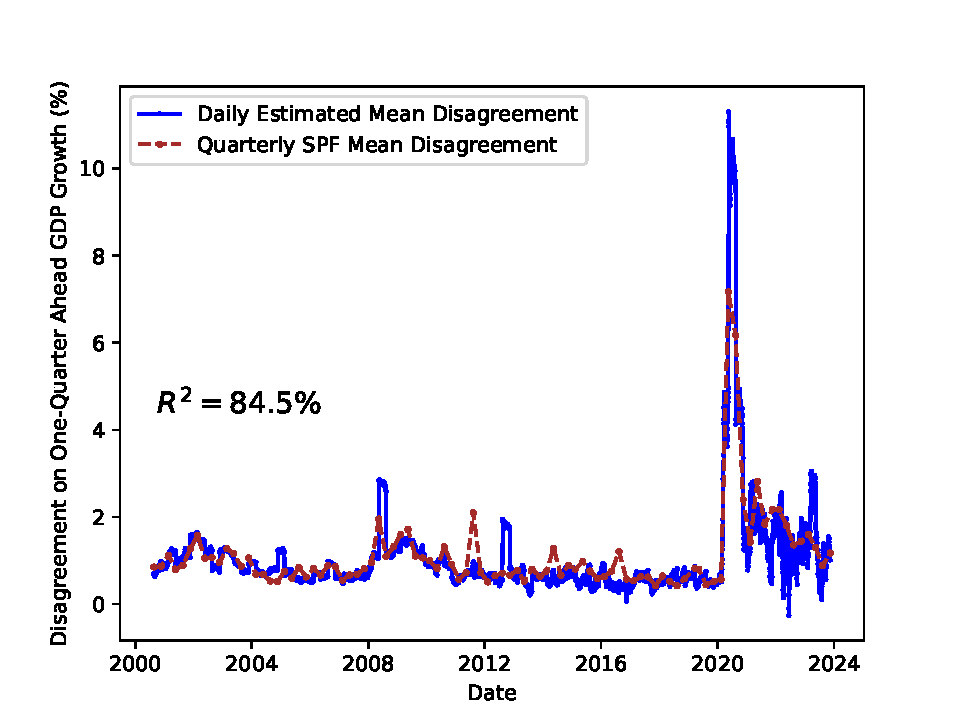
\includegraphics[width=0.8 \linewidth]
		    {pic/Figure_7.pdf}
		    \caption{Disagreement}
		  \end{center}
		\end{figure}
	\end{columns}
\end{frame}
\begin{frame}{Comparison with RL Approach: ML Interpretability}
	Both the RL method and our mixed-frequency method demonstrate strong empirical performance, realizing $R^2$ values of 82.3\% and 93.3\% for the cross-sectional mean, respectively.
	\\\ \\
	However, several important details warrant discussion:
	\begin{itemize}
		\item The RL method estimates the cross-sectional mean and variance jointly, which yields better estimates of the cross-sectional mean.
		\item Fixing $\alpha$ at one yields better performance than freely estimating $\alpha$.
		\item The parameters that the RL method needs to estimate are identical to those we consider, why we get different estimated results and empirical performance?
	\end{itemize}
\end{frame}

\section{Conclusion}
\begin{frame}{Conclusion}
	Main Findings:
	\begin{itemize}
		\item High-frequency dynamics of macro expectations and the corresponding evolution of disagreement among agents.
		\item A mixed-frequency framework that integrates high-frequency news with low-frequency survey data.
		\item Construction of daily time series for both cross-sectional mean and variance.
	\end{itemize}
	Future works:
	\begin{itemize}
		\item High-frequency series would enable clean identification in event studies.
		\item Our mixed-frequency framework can be applied to other macroeconomic variables to enhance the robustness of forecasting models.
	\end{itemize}
\end{frame}
%%%%%%%%%%%%%%%%%%%%%%%%%%
% End
\begin{frame}[allowframebreaks]%{End}
	\begin{center}
		\Huge\textbf{\textit{\texttt{Thanks!}}}
	\end{center}
\end{frame}

% Reference
%\appendix
%\begin{frame}{Reference}
%	\addtocounter{framenumber}{-1}
%	\printbibliography % [heading=bibintoc, title=Reference]
%\end{frame}

%%%%%%%%%%%%%%%%%%%%%%%%%%

% Snippets
%\begin{frame}[noframenumbering, plain]{Snippets}
%	\begin{multicols}{2}
%		\begin{enumerate}
%			\item \cite[Page10]{barro1990}
%			\item parencite \\ \parencite{Greiner2008}
%			\item footcite \footcite{green2020}
%			\item \cite{Greiner2008}
%		\end{enumerate}
%		\begin{itemize}
%			\item \[V = \frac{4}{3}\pi r^3\]
%			\item $ V = \frac{4}{3}\pi r^3 $
%		\end{itemize}
%	\end{multicols}	
%	\begin{equation}
%		\label{eq1}
%		V = \frac{4}{3}\pi r^3
%	\end{equation}
%	\center 
%	As Equation(\ref{eq1}) shows, $\cdots$, this \emph{equation} is \alert{important}.
%\end{frame}
%
%\begin{frame}[noframenumbering, plain]{Snippets}
%	\begin{columns}
%		\column{0.5\textwidth}
%			\begin{block}{Remark}
%				Sample text
%			\end{block}
%			\begin{alertblock}{Important theorem}
%				Sample text in red box
%			\end{alertblock}
%			\begin{examples}
%				Sample text in green box. 
%			\end{examples}
%		\column{0.5\textwidth}
%			\begin{table}
%			    \centering
%			    \caption{table1}
%			    \vspace{-0.5cm}
%			    \setlength{\tabcolsep}{5mm}
%				    {
%				    \begin{tabular}{lcc}
%				    \hline
%			        123 & 123 & ad f \\ \hline
%			        \textcolor{deepred}{123} & w & ad f \\ 
%			        \textcolor{sufered}{123} & \alert{ad} f & ad s f \\ \hline
%				    \end{tabular}
%				    }
%			    \label{fig1}
%			\end{table}
%	\end{columns}
%\end{frame}
%\backupend
%%%%%%%%%%%%%%%%%%%%%%%%%%
\end{CJK*}
\end{document}
